\chapter{Introdução}

\section{Contextualização do Problema}


% Na era atual de digitalização massiva, onde mais de 2.5 quintilhões de bytes \cite{gandomi2015137} são gerados diariamente, o crescimento acelerado de redes sociais e plataformas de e-commerce intensificou a demanda por métodos eficientes de classificação de textos. Essa necessidade não se restringe apenas à otimização da experiência do usuário, mas se estende a várias aplicações, incluindo filtragem de spam, análise de sentimento e personalização de publicidade \cite{alsmadi2019review}.

Na era atual de digitalização massiva, onde mais de 2.5 quintilhões de bytes \cite{gandomi2015137} são gerados diariamente, o crescimento acelerado de redes sociais e plataformas de e-commerce intensificou a demanda por métodos eficientes de classificação de textos. Esse vasto volume de dados exige sistemas automatizados que possam organizar e categorizar informações de maneira rápida e precisa, para otimizar a experiência do usuário e facilitar diversas aplicações, como filtragem de spam, análise de sentimento e personalização de publicidade \cite{alsmadi2019review}.


No contexto do idioma português, com suas particularidades, regionalismos e nuances entre variantes como o português do Brasil e de Portugal, a classificação textual apresenta desafios adicionais\cite{branco2012lingua}. Inclua-se o objetivo do trabalho, utilização de textos curtos, descrição curta é definida como um texto com até 200 caracteres, o que acrescenta uma camada de complexidade à tarefa, dado o conteúdo limitado disponível para análise \cite{alsmadi2019review} e \cite{song2014short}.

\subsection*{Exemplo do Problema de Categorização de Texto em Português}

Para ilustrar os desafios da categorização de textos curtos em português, considere a tarefa de identificar produtos da categoria "BISCOITO" em uma lista. A busca direta pela palavra "biscoito" retornaria resultados como "BISCOITO DUX SALGADO 648G" e "BISCOITO CRACKERS DUX 216G". No entanto, muitas descrições utilizam abreviações como "BISC LEITE MABEL 400G" e "BISC.PARATI MARIA PE 370GR", que seriam ignoradas pela busca simples.

Além disso, termos regionais ou estrangeiros como "BOLACHA", "COOKIE" e "COOKIES" também devem ser considerados, por exemplo, "BOLACHA PAPAGUARA MOTOR 400g" e "COOKIES GRAN CASTANH PARA KOBBER 150G". A complexidade aumenta quando produtos não relacionados são incluídos na busca, como "BISC PET CRACKER FORTAL 400G" (biscoitos para animais de estimação) e "CESTA SUPREME BISCOITO LIMAO 100G" (cesta de presentes), ou itens como camisetas com estampas que mencionam "BISCOITO".

\begin{figure}[h!]
    \begin{center}
    \caption{Camiseta com a palavra BISCOITO estampada}
    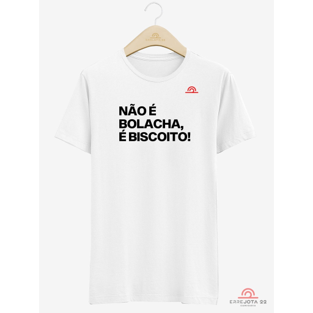
\includegraphics[scale=0.5]{images/camiseta.png}
    \label{fig:camiseta}
    \end{center}
\end{figure}

Esses exemplos demonstram a necessidade de métodos mais avançados para garantir uma classificação precisa.


% Suponha que se faz necessário encontrar, a partir de uma lista, todos os produtos que são da categoria "BISCOITO".  A primeira ideia é buscar por uma única palavra, por exemplo "biscoito".  Utilizando-se esta ideia encontra-se descrições como "BISCOITO DUX SALGADO 648G" e "BISCOITO CRACKERS DUX 216G".

% No entanto, há outras descrições de produtos onde "BISCOITO" é abreviado como "BISC LEITE MABEL 400G" e "BISC.PARATI MARIA PE 370GR", e esses resultados não seriam mostrados. Devido a este problema de abreviação e com o objetivo de realizar esta tarefa usando uma lista de palavras, seria necessário expandir a lista de palavras de busca para abranger as novas palavras "BISC" e "BISC." para serem reconhecidas como "BISCOITO".

% Também existem outras palavras completamente diferentes que deveriam retornar como resultado da busca por "BISCOITO". Essas palavras são, às vezes, termos locais ou estrangeiros e, novamente, precisaríamos expandir a lista de vocabulário. Por exemplo, "BOLACHA PAPAGUARA MOTOR 400g", "COOKIE INT BAUDUCCO AVEIA PASSAS 40G" e "COOKIES GRAN CASTANH PARA KOBBER 150G" onde as novas palavras são "BOLACHA", "COOKIE" e "COOKIES".

% Mesmo assim, essa solução aditiva não resolve completamente o problema, pois há algumas descrições contendo a palavra "BISCOITO", mas de fato não são. Por exemplo, "BISC PET CRACKER FORTAL 400G" e "BISC PET DOG CROCK 500G" são biscoitos para animais de estimação e "BISC LACTA BIS FLOWP 126G, LAKA BCO" e "CESTA SUPREME BISCOITO LIMAO 100G" são, respectivamente, chocolate e cesta de presentes. E uma camiseta estampada "NÃO É BOLACHA, É BISCOITO!" mostrada na Figura \ref{fig:camiseta} da mesma forma seria retornada pela pesquisa mas que não pertence a categoria desejada.

% \begin{figure}[h!]
%     \begin{center}
%     \caption{Camiseta com a palavra BISCOITO estampada}
%     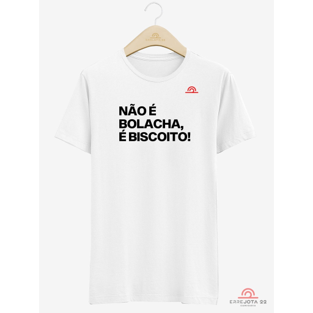
\includegraphics[scale=0.5]{images/camiseta.png}
%     \label{fig:camiseta}
%     \end{center}
%      %\small\textbf{Fonte:} Os autores.
% \end{figure}

% \section{Hipóteses}


% Diversas pesquisas têm indicado a variabilidade no desempenho dos algoritmos de aprendizado de máquina dependendo da técnica e do dataset em questão \cite{alsmadi2019review} e \cite{aggarwal2018review}. Técnicas de pré-processamento, como remoção de stopwords, stemming e lematização, podem ter um impacto significativo no desempenho dos modelos \cite{naseem2021survey}. Outro ponto a se considerar são os hiperparâmetros de cada modelo e sua otimização, que provocam significativas alterações nas medidas de avaliação de desempenho \cite{bhavani2021review}.

% \textbf{Hipótese:} Algoritmos de aprendizado de máquina, quando combinados com técnicas adequadas de pré-processamento e otimização de hiperparâmetros, podem melhorar significativamente a precisão, acurácia, recall e F1-score na classificação de descrições curtas de produtos em português.

\section{Hipóteses}

Diversas pesquisas têm indicado a variabilidade no desempenho dos algoritmos de recuperação da informação dependendo da técnica e do dataset em questão \cite{alsmadi2019review} e \cite{aggarwal2018review}. Técnicas de pré-processamento, como remoção de stopwords, stemming e lematização, podem ter um impacto significativo no desempenho dos modelos \cite{naseem2021survey}. Outro ponto a se considerar são os parâmetros de cada modelo e sua otimização, que provocam significativas alterações nas medidas de avaliação de desempenho \cite{bhavani2021review}.

\textbf{Hipótese:} Algoritmos simples de recuperação da informação, quando combinados com técnicas adequadas de pré-processamento e otimização de parâmetros, podem melhorar significativamente a precisão, acurácia, recall e F1-score na classificação de descrições curtas de produtos em português.



% Diversas pesquisas têm indicado a variabilidade no desempenho dos algoritmos de aprendizado de máquina dependendo da técnica e do dataset em questão \cite{alsmadi2019review} e \cite{aggarwal2018review}. Técnicas de pré-processamento, como remoção de stopwords, stemming e lematização, podem ter um impacto significativo no desempenho dos modelos\cite{naseem2021survey}. Outro ponto a se considerar são os hiperparâmetros de cada modelo e sua otimização provocam significativas alteração nas medidas de avaliação de desempenho \cite{bhavani2021review}.

% \section{Objetivos Gerais}

% O objetivo central deste estudo é analisar o desempenho, medido em termos de acurácia, precisão, recall e F1-score, de diferentes algoritmos de aprendizado de máquina na classificação de descrições curtas de produtos em português, utilizando o dataset DARU como referência.

% \subsection{Objetivos Específicos}

% Dentro deste escopo, busca-se:

% \begin{enumerate}
%     \item Avaliar o desempenho de algoritmos tradicionais e modernos, incluindo SVMs, regressão logística e redes neurais, na classificação de textos curtos.
%     \item Analisar o impacto de diferentes técnicas de pré-processamento, como remoção de stopwords, stemming e lematização, na eficácia dos modelos.
%     \item Determinar e otimizar os hiperparâmetros mais adequados para cada algoritmo.
% \end{enumerate}

\section{Objetivos Gerais}

O objetivo central deste estudo é analisar o desempenho, medido em termos de acurácia e F1-score macro, de diferentes algoritmos de recuperação da informação adaptados para a classificação de descrições curtas de produtos em português, utilizando o dataset DARU como referência.

\subsection{Objetivos Específicos}

Dentro deste escopo, busca-se:

\begin{enumerenumerate}
    \item Adaptar métodos de recuperação da informação, como sacola de palavras, TF e TF-IDF, para servirem como classificadores de descrições curtas de produtos.
    \item Avaliar o desempenho de algoritmos simples de recuperação da informação, como TF e TF-IDF com métricas de similaridade, na classificação de textos curtos em português.
    \item Analisar o impacto de diferentes técnicas de pré-processamento, como normalização e diferentes abordagens de tokenização, na eficácia dos modelos de recuperação da informação.
    \item Determinar e otimizar os parâmetros mais adequados para cada algoritmo, visando maximizar a acurácia e o F1-score macro.
    \item Adaptar uma métrica que unifique a acurácia e o F1-score macro para a avaliação de desempenho.
\end{enumerenumerate}

% \section{Justificativa e Relevância}

% A classificação apropriada de descrições de produtos é importante para a experiência do usuário, empresas e profissionais de e-commerce. Esta pesquisa, ao avaliar diferentes técnicas, oferece resultados consistentes para a área de processamento de linguagem natural e aprendizado de máquina, servindo como guia inicial para implementações mais eficazes.

\section{Justificativa e Relevância}

A classificação apropriada de descrições de produtos é relevante para a experiência do usuário, empresas e profissionais de e-commerce. Para os usuários, uma classificação eficiente facilita a busca por produtos, melhora a navegabilidade e personaliza as recomendações. Para as empresas, um sistema de classificação robusto otimiza a organização do catálogo de produtos, melhora a precisão das campanhas de marketing e aumenta a eficiência operacional.



% No contexto do idioma português, com suas particularidades, regionalismos e variações, a tarefa de classificação de textos curtos torna-se ainda mais desafiadora. Este estudo, ao adaptar e avaliar diferentes técnicas de recuperação da informação, oferece soluções práticas e aplicáveis para o mercado brasileiro, contribuindo para a melhoria das ferramentas de e-commerce e processamento de linguagem natural.


% \section{Metodologia}

% Nesta pesquisa, é adotada uma abordagem quantitativa para investigar o desempenho dos algoritmos de aprendizado de máquina na classificação de descrições curtas de produtos em português. O dataset DARU é utilizado como material principal, devido à sua relevância e abrangência no contexto brasileiro.

% A garantia da integridade e qualidade dos dados é obtida através da \textbf{Preparação dos Dados}. Esta etapa engloba o pré-processamento dos dados, no qual é feita a limpeza para remover qualquer inconsistência ou ruído, é realizada a remoção de stopwords - palavras comuns que podem não agregar valor significativo ao texto, e são aplicadas técnicas como stemming e lematização, que respectivamente reduzem as palavras à sua raiz e transformam palavras em sua forma base. Essa fase é essencial para assegurar que os algoritmos operem eficientemente e produzam resultados consistentes.

% Após a preparação, é realizada a \textbf{Seleção de Modelos}. Nesta etapa, são explorados diferentes algoritmos de aprendizado de máquina, desde abordagens tradicionais, como Máquinas de Vetores de Suporte (SVM) e regressão logística, até métodos mais contemporâneos como redes neurais. A escolha desses modelos é baseada em sua popularidade, eficácia comprovada e relevância para a tarefa de classificação de textos.

% Com os modelos selecionados, é feito o \textbf{Treinamento e Teste}. Os algoritmos escolhidos são treinados utilizando uma porção do dataset DARU. Para evitar o sobreajuste e garantir que os modelos tenham uma boa generalização, é empregada a técnica de validação cruzada estratificada. Esta abordagem envolve a divisão do dataset em múltiplos subconjuntos de forma que cada subconjunto seja usado tanto para treinamento quanto para teste, garantindo que todas as classes sejam representadas proporcionalmente.

% Finalmente, após o treinamento e teste dos modelos, é realizada a \textbf{Avaliação}. Nessa fase, o desempenho dos modelos é avaliado com base em métricas padrão, como acurácia, precisão, recall e F1-score. Estas métricas ajudam a entender o desempenho dos algoritmos, permitindo identificar os mais adequados para a tarefa em questão e fornecer insights sobre possíveis ajustes e otimizações.


\section{Metodologia}

Nesta pesquisa, é adotada uma abordagem quantitativa para investigar o desempenho dos algoritmos de recuperação da informação na classificação de descrições curtas de produtos em português. O dataset DARU é utilizado como material principal, devido à sua relevância e abrangência no contexto brasileiro.

\subsection{Preparação dos Dados}
A garantia da integridade e qualidade dos dados é obtida através do pré-processamento dos dados. Esta etapa inclui a limpeza para remover inconsistências ou ruído, normalização para padronizar os textos, e a aplicação de diferentes abordagens de tokenização. Essas técnicas asseguram que os algoritmos operem eficientemente e produzam resultados consistentes.

\subsection{Seleção e Adaptação de Algoritmos}
Nesta etapa, são adaptados diferentes métodos de recuperação da informação, como sacola de palavras, TF e TF-IDF, para servirem como classificadores. A adaptação envolve agrupar as descrições em um documento, onde cada documento representa uma categoria, e a aplicação de métricas de similaridade para determinar a categoria mais provável de cada descrição de produto.

\subsection{Treinamento e Teste}
Os algoritmos escolhidos são treinados utilizando uma porção do dataset DARU. Para evitar o sobreajuste e garantir uma boa generalização, é empregada a técnica de validação cruzada estratificada. Esta abordagem envolve a divisão do dataset em múltiplos subconjuntos, garantindo que todas as classes sejam representadas proporcionalmente.

\subsection{Avaliação}
O desempenho dos modelos é avaliado com base em métricas padrão, como acurácia e F1-score macro. Estas métricas ajudam a entender o desempenho dos algoritmos, permitindo identificar os mais adequados para a tarefa em questão e fornecer insights sobre possíveis ajustes e otimizações.

\subsection{Proposta de Métrica Unificada}
Além das métricas padrão, é proposto a adaptação de uma métrica que unifique a acurácia e o F1-score macro para a avaliação de desempenho dos algoritmos de recuperação da informação.

% \section{Contribuições}

% As principais contribuições deste trabalho são:

% \begin{itemize}
%     \item Uma análise aprofundada do desempenho de diferentes algoritmos de aprendizado de máquina na classificação de textos curtos em português.
%     \item Diretrizes sobre as técnicas de pré-processamento mais eficazes para esta tarefa.
%     \item Recomendações para otimização de hiperparâmetros para diferentes algoritmos.
% \end{itemize}

\section{Contribuições}

As principais contribuições deste trabalho são:

\begin{itemize}
    \item Uma análise aprofundada do desempenho de diferentes algoritmos de recuperação da informação na classificação de textos curtos em português.
    \item Diretrizes sobre as técnicas de pré-processamento mais eficazes para esta tarefa.
    \item Recomendações para otimização de parâmetros para diferentes algoritmos de recuperação da informação.
    \item Adaptação de uma métrica unificada que combina acurácia e F1-score macro.
\end{itemize}


% \section{Estrutura do Trabalho}

% Este trabalho é estruturado da seguinte forma:

% \begin{enumerate}
%     \item \textbf{Introdução:} Contextualização do problema, objetivos, justificativa e relevância.
%     \item \textbf{Revisão Literária:} Discussão sobre trabalhos anteriores, técnicas e algoritmos relevantes.
%     \item \textbf{Metodologia:} Descrição detalhada da abordagem adotada na pesquisa.
%     \item \textbf{Resultados:} Apresentação e discussão dos resultados obtidos.
%     \item \textbf{Conclusão:} Resumo dos achados, contribuições e sugestões para trabalhos futuros.
% \end{enumerate}

\section{Estrutura do Trabalho}

Este trabalho é estruturado da seguinte forma:

\begin{enumerate}
    \item \textbf{Introdução:} Contextualização do problema, objetivos, justificativa e relevância.
    \item \textbf{Revisão Literária:} Discussão sobre trabalhos anteriores, técnicas e algoritmos relevantes.
    \item \textbf{Metodologia:} Descrição detalhada da abordagem adotada na pesquisa, incluindo a adaptação de algoritmos de recuperação da informação.
    \item \textbf{Resultados:} Apresentação e discussão dos resultados obtidos.
    \item \textbf{Conclusão:} Resumo dos achados, contribuições e sugestões para trabalhos futuros.
\end{enumerate}



% \section{CIMO - Contexto, Problema, Objetivo, Método e Contribuição}

% \subsection{Contexto}
% Na era atual de digitalização massiva, a classificação textual tornou-se uma ferramenta essencial, especialmente no domínio do e-commerce e redes sociais. Com a crescente quantidade de dados gerados diariamente, métodos eficazes de categorização são cruciais.

% \subsection{Problema}
% Dada a rica complexidade do idioma português e a necessidade de classificar textos curtos, como descrições de produtos, existe uma demanda por algoritmos de aprendizado de máquina eficientes e precisos para esta tarefa.

% \subsection{Objetivo}
% O estudo visa analisar e otimizar o desempenho de diferentes algoritmos de aprendizado de máquina na classificação de descrições curtas de produtos em português.

% \subsection{Método}
% Serão utilizados diversos algoritmos, desde abordagens tradicionais até técnicas mais modernas, avaliando o impacto de diferentes técnicas de pré-processamento e otimização de hiperparâmetros.

% \subsection{Contribuição}
% Esta pesquisa espera contribuir para a área de processamento de linguagem natural e aprendizado de máquina, fornecendo diretrizes e práticas recomendadas para a classificação de textos curtos em português.

\section{CIMO - Contexto, Problema, Objetivo, Método e Contribuição}

\subsection{Contexto}
Na era atual de digitalização massiva, a classificação textual tornou-se uma ferramenta essencial, especialmente no domínio do e-commerce e redes sociais. Com a crescente quantidade de dados gerados diariamente, métodos eficazes de categorização são necessários.

\subsection{Problema}
Dada a complexidade do idioma português e a necessidade de classificar textos curtos, como descrições de produtos, existe uma demanda por algoritmos de recuperação da informação eficientes e precisos para esta tarefa.

\subsection{Objetivo}
O estudo visa analisar e otimizar o desempenho de diferentes algoritmos de recuperação da informação na classificação de descrições curtas de produtos em português.

\subsection{Método}
Serão utilizados diversos algoritmos de recuperação da informação, como sacola de palavras, TF e TF-IDF, avaliando o impacto de diferentes técnicas de pré-processamento e otimização de parâmetros.

\subsection{Contribuição}
Esta pesquisa espera contribuir para a área de processamento de linguagem natural, fornecendo diretrizes e práticas recomendadas para a classificação de textos curtos em português, além de adaptar uma métrica unificada que combina acurácia e F1-score macro.
